\documentclass{beamer}

%Packages
\usepackage[utf8]{inputenc}
\usepackage{hyperref}

% Hide navigation symbols, show git
\setbeamertemplate{navigation symbols}{}
\setbeamertemplate{footline}[frame number]

\newcommand{\inote}[1]{
  {
    \begin{itemize}
      \item #1
    \end{itemize}
  }
}

% Logos
\newcommand{\logoimage}[2]{\begingroup
\setbox0=\hbox{\includegraphics[height=#2]{#1}}%
\parbox{\wd0}{\box0}\endgroup\ }

% Have a fancy git logo
\newcommand{\git}{\logoimage{imgs/git_logo}{10pt}}
\newcommand{\github}{\logoimage{imgs/github_logo}{10pt}}

%META-INFORMATION
\title{\logoimage{imgs/git_logo}{40px} - the content tracker}
\author{Tom Wiesing}
\institute{CS Club}
\date{September 5, 2015}

\begin{document}
    %TITLEPAGE
    \frame{\titlepage}
    
    \begin{frame}{Overview}
      \begin{itemize}
          \item Introduction: What is version control and why use git?
          \item Getting started: The git model
          \item Using git: clone, init, add, commit, push, pull
          \item Going further: Branching, Merging, Stashing and more
          \item \github: Collaboration with Issues, Forking, Pull Requests
          \item Behind the Scenes: Internals of Git
          \item Demo / Hacking / Questions
      \end{itemize}
    \end{frame}

    %intro - what is version control and why git?
    \begin{frame}{Introduction (1): What is version control?}
      \begin{columns}[onlytextwidth]
        \begin{column}{0.6\textwidth}
          \begin{itemize}
              \item tracks any kind of content
                \inote{e.g. websites, software, presentations}
              \item knows about different versions
              \begin{itemize}
                \item knows what was changed when
                \item can revert changes if something goes wrong
              \end{itemize}
              \item has a collaboration component
              \begin{itemize}
                \item several people can work together on the same project
                \item changes can be synced
                \item easy to see who changed what
              \end{itemize}
            \end{itemize}
        \end{column}
        \begin{column}[t]{0.4\textwidth}
          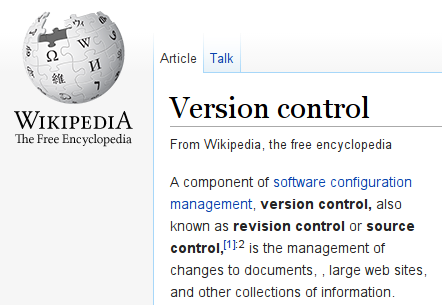
\includegraphics[width=0.95\textwidth]{imgs/vc_wikipedia}
        \end{column}
      \end{columns}
    \end{frame}
    
    \begin{frame}{Introduction (2): What is git and why use it?}
      \begin{columns}[onlytextwidth]
        \begin{column}{0.6\textwidth}
          \begin{itemize}
            \item git -- ``the stupid content tracker''
            \begin{itemize}
              \item open-source version control system
              \item fast, scalable, distributable
            \end{itemize}
            \item originally developed in 2005 for maintaining the linux kernel source code
          \end{itemize}
        \end{column}
        \begin{column}[t]{0.4\textwidth}
          
\includegraphics[width=0.95\textwidth]{imgs/git_logo}
        \end{column}
      \end{columns}
    \end{frame}
    
    \begin{frame}{Introduction (3): What is git and why use it?}
      \begin{itemize}
        \item git is both for beginners and advanced users
        \begin{itemize}
          \item provides high-level-commands
          \item additonally gives full access to internals
        \end{itemize}
        \item git is distributed - and it is easy to sync changes
        \begin{itemize}
          \item no central server to share content required
          \item changes can be synced in many ways
          \item[] {\tiny \hfill http(s), ssh, git protocol, diffs via email, \dots}
        \end{itemize}
      \end{itemize}
    \end{frame}
    
\end{document}
